\documentclass[a4paper]{article}
\usepackage{enumitem, amsmath, gensymb, graphicx, caption, amssymb, geometry, fancyhdr, arydshln, adjustbox}

\geometry{left=1in, right=1in, top=1in, bottom=1in}
\pagestyle{fancy}

\newcommand{\myName}{\textbf{Shantanu Ghodgaonkar}\\\textit{Univ ID}: N11344563\\\textit{Net ID}: sng8399\\\textit{Ph.No.}: +1 (929) 922-0614}
\newlist{qalist}{description}{1}
\setlist[qalist]{style=unboxed,leftmargin=0.5cm,labelwidth=2.5cm}


\title{Homework 2 Answers : ROB-GY 6003}
\author{\myName}
\date{\today}

\fancyhead{} % Clear existing header settings 
\fancyhead[L]{\today}
\fancyhead[R]{N11344563}


\begin{document}
	
	\begin{titlepage}
	    \centering
	    \vspace{2cm}
	    \Huge\textbf{Foundations of Robotics \\ ROB-GY 6003 \\ Homework 3 Answers}
	    \vspace{1cm}
	    \\ \Large \today
	    \vfill 
	    \Large \myName
	\end{titlepage}
	
	\begin{qalist}			
		\item[Question: 4.8] \setcounter{equation}{0} %12
		\item[Answer:] Given a desired position and orientation of the hand of a four-link planar rotary-jointed manipulator, there are an infinite number of possible solutions. This is because an added degree of freedom would allow for an infinite number of positions and orientations of the links between the wrist and the base, assuming that the position of the wrist were fixed. 
			
		\item[Question: 4.9] \setcounter{equation}{0} %26
		\item[Answer:] Here is what the approximate \textit{reachable workspace} of the given robot would look like - 
			\begin{figure}[h!]			
				\vspace{0.5cm}
				\centering
				\fbox{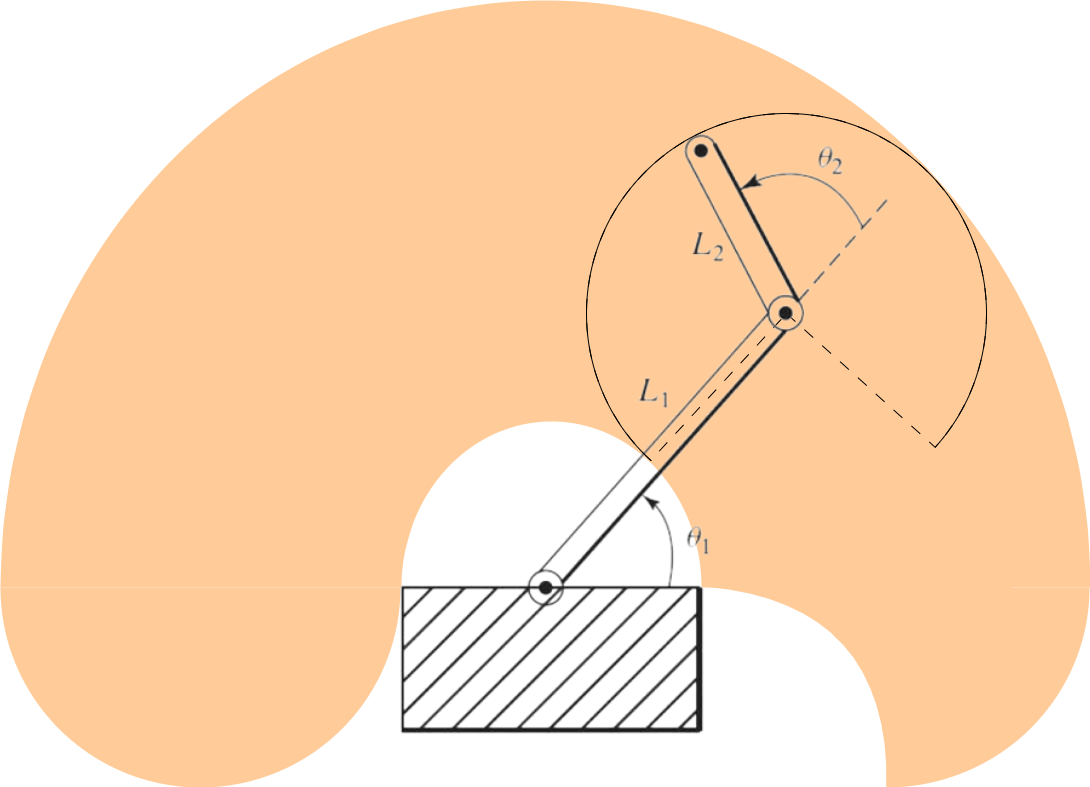
\includegraphics[width=0.75\textwidth]{q4_9.png}}
				\caption{Two-link planar manipulator \textit{Reachable Workspace}} 
				\label{fig:q4_9}
				\vspace{0.5cm}
			\end{figure}
		\\The orange highlight represents the \textit{reachable workspace} whereas the arc represents the motion of the tip of ${L}_{2}$.
		\item[Question: 4.18] \setcounter{equation}{0} %15
		\item[Answer:] There are 2 possible solutions to the kinematic equations.
		
		\item[Question: 4.19] \setcounter{equation}{0} %15
		\item[Answer:] There are 4 possible solutions to the kinematic equations.
		
		\item[Question: 4.24] \setcounter{equation}{0} %20
		\item[Answer:] The DH parameters as functions of the elements of ${}^{i-1}_{i}T$ can be written as, 
			\begin{align}
				{\theta}_{i-1} &= {T}_{14}\\
				{\theta}_{i} &= atan2(-{T}_{12}, {T}_{11})\\
				{d}_{i} &= \sqrt{{T}^{2}_{24}+{T}^{2}_{34}}\\
				{a}_{i-1} &= {T}_{14}\\ 
				{\alpha}_{i-1} &= atan2(-{T}_{23}, {T}_{33})
			\end{align}
	\end{qalist}
\end{document}